\documentclass[12pt]{article}%
\usepackage[paper=portrait,pagesize]{typearea}
\usepackage{amssymb}
\usepackage{amsfonts}
\usepackage{amsmath}
\usepackage{hyperref}
\usepackage{lscape}
\usepackage{comment}
\usepackage[flushleft]{threeparttable}
\usepackage{float}
\usepackage[nohead]{geometry}
\usepackage[singlespacing]{setspace}
\usepackage[paper=portrait,pagesize]{typearea}
\usepackage{amssymb}
\usepackage{amsfonts}
\usepackage{multicol}
\usepackage{amsmath}
\usepackage{hyperref}
\usepackage[nameinlink,noabbrev]{cleveref}
\usepackage{lscape}
\usepackage{float}
\usepackage[nohead]{geometry}
\usepackage[singlespacing]{setspace}
\usepackage[bottom]{footmisc}
\usepackage{indentfirst}
\usepackage{endnotes}
\usepackage{graphicx}%
\usepackage{afterpage}
\usepackage{subfig}
\usepackage{rotating}
\newcommand\tab[1][1cm]{\hspace*{#1}}
\DeclareMathOperator*{\Max}{Max}
\newcommand\numberthis{\addtocounter{equation}{1}\tag{\theequation}}
\def\dotfill#1{\cleaders\hbox to #1{.}\hfill}
\newcommand\dotline[2][.5em]{\leavevmode\hbox to #2{\dotfill{#1}\hfil}}
%\usepackage[backend=biber,style=alphabetic,sorting=ynt]{biblatex}
%\addbibresource{bibliocopulas.bib}
\usepackage[round,sort,comma,authoryear]{natbib}
\setcounter{MaxMatrixCols}{30}
\newtheorem{theorem}{Theorem}
\newtheorem{acknowledgement}{Acknowledgement}
\newtheorem{algorithm}[theorem]{Algorithm}
\newtheorem{axiom}[theorem]{Axiom}
\newtheorem{case}[theorem]{Case}
\newtheorem{claim}[theorem]{Claim}
\newtheorem{conclusion}[theorem]{Conclusion}
\newtheorem{condition}[theorem]{Condition}
\newtheorem{conjecture}[theorem]{Conjecture}
\newtheorem{corollary}[theorem]{Corollary}
\newtheorem{criterion}[theorem]{Criterion}
\newtheorem{definition}[theorem]{Definition}
\newtheorem{example}[theorem]{Example}
\newtheorem{exercise}[theorem]{Exercise}
\newtheorem{lemma}[theorem]{Lemma}
\newtheorem{notation}[theorem]{Notation}
\newtheorem{problem}[theorem]{Problem}
\newtheorem{proposition}{Proposition}
\newtheorem{remark}[theorem]{Remark}
\newtheorem{solution}[theorem]{Solution}
\newtheorem{summary}[theorem]{Summary}
\newenvironment{proof}[1][Proof]{\noindent\textbf{#1.} }{\ \rule{0.5em}{0.5em}}
\newcommand{\pd}[2]{\frac{\partial#1}{\partial#2}}
\makeatletter
\def\@biblabel#1{\hspace*{-\labelsep}}
\makeatother
\geometry{left=1in,right=1in,top=1.00in,bottom=1.0in}
%\renewcommand*\abstractname{Summary}

\begin{document}

\title{Fall 2019 - ECON 634 - Advance Macroeconomics - Problem Set 3}
\author{Elisa Taveras Pena\footnote{E-mail address: \href{mailto:etavera2@binghamton.edu}{etavera2@binghamton.edu}  }\\
Binghamton University}
\maketitle

\sloppy%avoids the breakage of words at the end of lines, by adjusting spaces between words inside the lines

\onehalfspacing

\begin{enumerate}
	\item	We can write the budget constraint  in recursive form as  $c=y(s)+a -qa'$ 
	
	\tab \textbf{ $\bullet$ State variable}: $a,s$ 
	
	\tab \textbf{ $\bullet$ Control variable}: $a'$
	
	
	
	Therefore, the Bellman equation:
	
	\begin{align*}
	&V(a,s)=\Max_{a'\in \Gamma(a,s)} \left\lbrace \frac{\left( y(s)+a -qa'\right) ^{1-\sigma}}{1-\sigma}+ \beta \sum_{s' \in S} \Pi(s'|s)V(a',s')\right\rbrace 
	& \notag \\
	&\text{subject to} \notag \\
	& \tab \Gamma(a,s) \in \left[ 0,f(k)\right] \numberthis\\
	\end{align*} 
	
	\item The Risk free price is \textbf{0.9950}.
	
	\item The Lorenz curve looks as follows:
	
	\begin{center}
		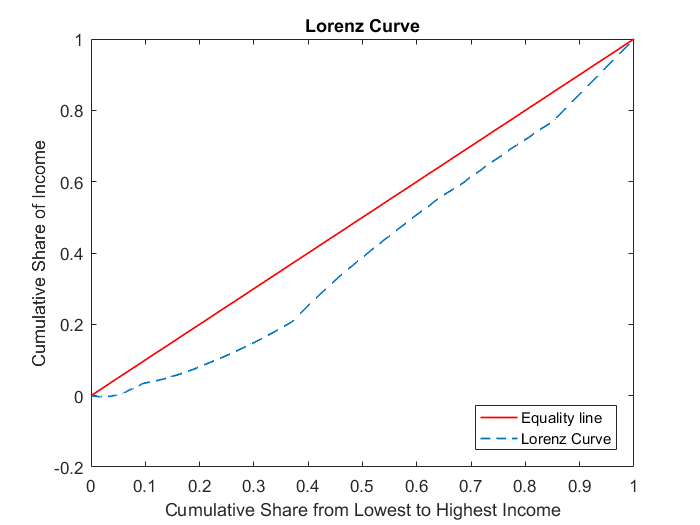
\includegraphics[width=1\linewidth]{Lorenz}
	\end{center}
	
	\item Extra credit:
	
	\begin{itemize}
		\item If everyone started out with zero assets, and there was perfect insurance against all income shocks, what would the allocation be? What would be expected utility of that allocation?
		
		\vspace{1mm}
		
		If everyone can perfectly insurance against all the shock, and because there is no aggregate uncertainty, they will consume the same in each period (consumption smoothness). This means that in each period, they consume the expected value of their endowment (expected wages). This means that:
		
			\begin{align*}
		\bar{c}=\pi_{e}y(e)+\pi_{u}y(u)={0.9434}(1)+{0.0566}(.5)=0.9717  \tab  \forall t \notag \\ 				
		\end{align*}
		
		Then, the expected Utility of this consumption is: 
				\begin{align*}
		&W^{FB}(\bar{c})={\sum}_{t=0}^{\infty}\beta^{t}\frac{\bar{c}_e^{1-\sigma}}{1-\sigma}=\frac{\bar{c}_e^{1-\sigma}}{1-\sigma}\frac{1}{1-\beta}= -338.1529\\		 
		\end{align*}
		
		\vspace{1mm}
		
		\item Which fraction of households would benefit from that plan?
			
		\vspace{1mm}
		
		100\% of the household are made better off by the government plan.	
		
		
		\item Welfare Gain?
			\vspace{1mm}
		
	 There is complete economic welfare gain which is equal to $0.0027$, which means that we offer consumption.
		
		
	\end{itemize}
	
\end{enumerate}

\strut

\onehalfspacing

\end{document}
